\documentclass[11pt,a4paper]{article}

\usepackage[utf8]{inputenc}
\usepackage[T1]{fontenc}
\usepackage{lmodern}
\usepackage[margin=1in]{geometry}
\usepackage{amsmath,amssymb,amsthm}
\usepackage{booktabs}
\usepackage{enumitem}
\usepackage{listings}
\usepackage{xcolor}
\usepackage{float}
\usepackage{tikz}
\usetikzlibrary{arrows.meta,positioning,calc}
\usepackage[colorlinks=true,linkcolor=blue,citecolor=blue,urlcolor=blue]{hyperref}

% Theorem environments
\newtheorem{theorem}{Theorem}
\newtheorem{definition}{Definition}
\newtheorem{proposition}{Proposition}
\newtheorem{claim}{Claim}

% Custom macros
\newcommand{\Stau}{S_\tau}
\newcommand{\deff}{d_{\mathrm{eff}}}

% Futuruna language listings
\definecolor{runagreen}{RGB}{0,128,0}
\definecolor{runagray}{RGB}{100,100,100}
\definecolor{runaorange}{RGB}{200,80,0}
\definecolor{runablue}{RGB}{0,60,160}
\definecolor{runabg}{RGB}{248,248,248}

\lstdefinelanguage{runa}{
  keywords={match, if, else, for, in, with, under, exception, self, true, false},
  keywordstyle=\color{runablue}\bfseries,
  morecomment=[l]{--},
  commentstyle=\color{runagreen}\itshape,
  stringstyle=\color{runaorange},
  morestring=[b]",
  sensitive=true,
  literate=
    {->}{{$\rightarrow$}}2,
}

% Rust listings for comparison
\lstdefinelanguage{rustlang}{
  keywords={fn, let, struct, enum, impl, pub, mut, self, match, if, else, for, in, use, mod, trait, where, return, type, const, static, ref, move, async, await, dyn, Box, Vec, String, Option, Result, Some, None, Ok, Err, true, false},
  keywordstyle=\color{runablue}\bfseries,
  morecomment=[l]{//},
  commentstyle=\color{runagreen}\itshape,
  stringstyle=\color{runaorange},
  morestring=[b]",
  sensitive=true,
  literate=
    {->}{{$\rightarrow$}}2,
}

\lstset{
  language=runa,
  basicstyle=\small\ttfamily,
  backgroundcolor=\color{runabg},
  frame=single,
  framerule=0.4pt,
  rulecolor=\color{gray!50},
  numbers=none,
  xleftmargin=6pt,
  xrightmargin=6pt,
  aboveskip=8pt,
  belowskip=8pt,
  breaklines=true,
  columns=fullflexible,
  keepspaces=true,
  showstringspaces=false,
  tabsize=4,
}

\title{\textbf{Futuruna: The Seven Symbols That Creates\\Clear Programming Without Compromise}}
\author{Andreas Rudolph\\Independent researcher, Copenhagen}
\date{}

\begin{document}
\maketitle

\begin{abstract}
You open a file in an unfamiliar language. Within seconds, before you understand a single line, something in you either relaxes or tightens. That feeling has a number. We measured it for every major programming language and found that the syntax of every one of them answers at most two questions before you read a single word. You passively know how deep you are in nested blocks, and perhaps whether you are in a type or an expression. Everything else requires decoding: you read the keyword \texttt{fn} to learn it is a function, \texttt{struct} to learn it is a type.

A single innovation opens a third question. Place a dedicated character at the very start of each line, one that declares what kind of statement follows. We call this character a \emph{rune}. The resulting language, Futuruna, has seven: \texttt{\#}~what exists, \texttt{>}~what happens, \texttt{|}~what must be true, \texttt{=}~what is, \texttt{\textasciitilde}~what flows, \texttt{@}~where proofs stop, \texttt{?}~prove it. Now the syntax passively tells you the statement kind, the type flow, and the block depth. Three questions answered for free.

We formalize this using three information-theoretic quantities: \emph{optionality} (how many continuations exist), \emph{clarity} (how distinguishable positions are), and \emph{integration} (how many independent questions the syntax answers at once). Every existing language scores at most two on integration. Futuruna scores three. It compiles to native Rust with inferred ownership, unifies logic programming with pattern matching with legal default logic under one character, and provides a Z3 verification pipeline where each rune maps directly to a category in the formal methods backend.
\end{abstract}

\medskip
\noindent\textbf{Keywords:} programming language design, integrated information theory, causal entropic forces, statement runes, formal verification, cognitive dimensionality

%% ============================================================================
\section{Imagine}
%% ============================================================================

Imagine a program where types, functions, rules, values, streams, effects, and verification are each announced by a single character at the start of the line:

\begin{lstlisting}
# Condition = Sunny | Cloudy | Stormy
# Weather(day: String, temp: Float, condition: Condition)

> describe(w: Weather) -> String {
    match w.condition {
        | Sunny -> show(w.temp) + " C, sunny"
        | Stormy -> show(w.temp) + " C, storm"
        | Cloudy -> show(w.temp) + " C, cloudy"
    }
}

| advisory(w) -> "all clear"
| advisory(w) -> "heat warning" under w.temp > 35.0
| exception storm advisory(w) -> "danger" under w.condition == Stormy

= today = Weather("today", 22.0, Sunny)
= alert = advisory(today)

@ print(today.day + ": " + describe(today) + " -- " + alert)

~ forecast = from_list([today, Weather("tomorrow", 40.0, Sunny),
    Weather("in 2 days", 18.0, Cloudy), Weather("in 3 days", 10.0, Stormy)])
    |> filter(|w: Weather| advisory(w) != "all clear")

= warning_count = count(forecast)
| has_warnings: warning_count -> warning_count > 0

? has_warnings: n -> {
    @ print("Upcoming warnings (" + show(n) + "):")
    ~ forecast | w -> {
        @ print("  " + w.day + ": " + advisory(w) + " -> " + describe(w))
    }
} else {
    @ print("No warnings -- all clear ahead")
}
\end{lstlisting}

\noindent The output:
\begin{verbatim}
today: 22.0 C, sunny -- all clear
Upcoming warnings (2):
  tomorrow: heat warning -> 40.0 C, sunny
  in 3 days: danger -> 10.0 C, storm
\end{verbatim}

Seven runes, and they feed into each other. \texttt{\#} defines types that every other rune uses. \texttt{>} defines \texttt{describe}, a function with \texttt{|} match arms inside. Three \texttt{|} lines define \texttt{advisory} as rules with override logic: the default is ``all clear,'' high temperature overrides to ``heat warning,'' storms override everything---no \texttt{if/else} chain, no Prolog. Notice the output: four days go in, but only two warnings come out. Day two (18\textdegree C, cloudy) triggers no override rule, so the default ``all clear'' holds and the filter silently removes it. The logic rules did the work; the stream carried the result. \texttt{=} binds \texttt{today} and calls the rules to get \texttt{alert}. \texttt{@} prints by combining the function and rule results. \texttt{\textasciitilde} declares a reactive stream that pipes \texttt{today} (an \texttt{=} binding) through a filter that calls the \texttt{|} rules---showing values flowing between runes. Then \texttt{|} appears again as a named invariant, and \texttt{?} interrogates it: \texttt{?~has\_warnings: n} captures the checked value, runs the pass block when it holds, and falls through to \texttt{else} when it does not.

Count the \texttt{|} character: it appears as match arms, as logic rules with exceptions, and as a named invariant that \texttt{?} interrogates. Three roles, one symbol, because they are all the same operation: \emph{case analysis}.

A \emph{rune} is a single special character placed at the very start of a line to declare what kind of statement follows. Futuruna has seven of them. Each one answers the same question: \emph{what am I about to tell you?}

\begin{center}
\texttt{\#}~what exists \quad \texttt{>}~what happens \quad \texttt{|}~what must be true \quad \texttt{=}~what is\\[3pt]
\texttt{\textasciitilde}~what flows \quad \texttt{@}~where proofs stop \quad \texttt{?}~prove it
\end{center}

In every existing language, you read the first \emph{word} of a line to know what kind of statement it is: \texttt{fn}, \texttt{let}, \texttt{struct}, \texttt{if}, \texttt{println!}. In Futuruna, you read the first \emph{character}. In the listing above, your eye scans \texttt{|}, \texttt{\#}, \texttt{>}, \texttt{=}, \texttt{\textasciitilde}, \texttt{@}, \texttt{?} and knows what each line does before processing a single identifier.

That difference has a number. We call it $\deff$: how many independent questions the syntax answers for free. In a language with $\deff = 1$, you passively know one thing: how deep you are in nested blocks. Everything else requires reading. In a language with $\deff = 3$, you passively know three things: what \emph{kind} of statement you are on, what \emph{types} flow through it, and where it \emph{sits} in the structure. Three facts, delivered through three independent visual cues, before your brain processes a single word.

Every existing language scores $\deff \leq 2$. Futuruna scores $\deff = 3$.

%% ============================================================================
\section{What One Rune Replaces}
%% ============================================================================

Before the theory, look at what collapses.

\begin{table}[H]
\centering
\caption{Each rune absorbs mechanisms scattered across multiple keywords and languages.}
\label{tab:unifies}
\small
\begin{tabular}{clp{8cm}}
\toprule
Rune & Unifies & Scattered across \\
\midrule
\texttt{\#} & Types + Effects + Traits & \texttt{class}, \texttt{struct}, \texttt{enum}, \texttt{interface}, \texttt{trait}, \texttt{type} \\
\texttt{>} & Functions + Actors + Modules & \texttt{fn}, \texttt{def}, \texttt{func}, \texttt{mod}, \texttt{actor} \\
\texttt{|} & Logic + Matching + Effects + Law & Prolog (\texttt{:-}), Rust (\texttt{match}), Koka (\texttt{handle}), Catala (\texttt{rule}) \\
\texttt{=} & Binding + Monadic bind & \texttt{let}, \texttt{val}, \texttt{var}, Haskell \texttt{<-} \\
\texttt{\textasciitilde} & Reactive streams & RxJS, Reactor, Akka Streams (libraries, not language) \\
\texttt{@} & IO + Imports + Build + FFI & \texttt{println!}, \texttt{use}, \texttt{import}, \texttt{build.gradle}, FFI \\
\texttt{?} & Tests + Asserts + Formal proofs & \texttt{assert!}, \texttt{\#[test]}, external Z3 toolchain \\
\bottomrule
\end{tabular}
\end{table}

The \texttt{|} row is the headline. Today, if you want logic programming, you learn Prolog. If you want legal rules with exceptions that override defaults, you learn Catala. If you want algebraic effects (a way to declare side effects like IO and state as values the caller can intercept and handle), you learn Koka. If you want pattern matching, you learn Rust or Haskell. Four different languages for four instances of the same idea: \emph{case analysis under different regimes}.

In Futuruna, they are one rune.

\begin{lstlisting}
-- Prolog-style inference
| taxable(person) -> resident(person), has_income(person)

-- Catala-style default logic with exceptions
| tax_rate(person) -> 0.20
| tax_rate(person) -> 0.40 under person.income > 50000
| exception tax_rate(person) -> 0.00 under person.income < 12000

-- Koka-style algebraic effect handler
| handle Console {
    | say(msg) -> { @ print(msg); resume(()) }
    | ask(prompt) -> resume("default")
} in greet("World")

-- ML-style pattern matching
match shape {
    | Circle(r) -> 3.14 * r * r
    | Rectangle(w, h) -> w * h
}
\end{lstlisting}

Four capabilities. One character. The reason they unify is structural: they are all case analysis. Logic clauses analyze cases over a search space. Pattern matching analyzes cases of a value. Effect handlers analyze cases of a side effect. Legal rules analyze cases of a regulation. The regimes differ. The operation does not.

\subsection{The ownership problem, dissolved}

Here is a function in Rust:

\begin{lstlisting}[language=rustlang]
fn process(data: &[String], prefix: &str) -> Vec<String> {
    data.iter()
        .filter(|s| s.starts_with(prefix))
        .map(|s| s.clone())
        .collect()
}
\end{lstlisting}

The programmer had to decide: \texttt{\&[String]} or \texttt{Vec<String>}? \texttt{\&str} or \texttt{String}? \texttt{s.clone()} or \texttt{s.to\_string()}? Every one of those decisions is an ownership annotation that Rust requires and the programmer provides.

Here is the same function in Futuruna:

\begin{lstlisting}
> process(data: List(String), prefix: String) -> List(String) {
    filter(data, |s| starts_with(s, prefix))
}
\end{lstlisting}

No \texttt{\&}. No lifetime. No \texttt{.clone()}. The compiler sees that \texttt{data} is read-only and emits \texttt{\&[String]} automatically. It sees that \texttt{prefix} is only borrowed and emits \texttt{\&str}. It sees the filter closure captures by reference and skips the clone. The generated Rust is identical to---or better than---what a careful programmer would write.

In an adversarial comparison of 12 ownership patterns that commonly trip Rust newcomers, Futuruna produces valid Rust for all 12. It wins on 5 (zero clones where Rust requires manual annotation), ties on 7, loses on none.

\subsection{Verification as syntax}

The \texttt{?} rune scales from runtime check to formal proof without changing the source code:

\begin{lstlisting}
| conservation: supply -> supply >= 0 && supply <= max_supply
? conservation
\end{lstlisting}

In the interpreter, \texttt{?~conservation} evaluates the predicate with current values. In compiled mode, it emits \texttt{debug\_assert!()}. With \texttt{runa verify}, it translates the invariant into a format for automated theorem provers and invokes Z3 \cite{DeMoura2008} (Microsoft's open-source theorem prover) to prove the invariant holds for \emph{all} inputs. One character. Three levels of assurance. The code never changes.

%% ============================================================================
\section{The Measurement}
%% ============================================================================

The claims above are not aesthetic opinions. One character changes how you navigate code. Futuruna occupies a region of design space no existing language touches. Both claims are the result of applying two theories from outside computer science to the structure of programming language syntax.

\subsection{What we measured}

Take any programming language. Collect a representative corpus of code. Classify every token into one of 22 categories---keyword, identifier, type name, operator, brace, parenthesis, and so on. Count how often each category follows each other. Normalize to probabilities. The result is a $22 \times 22$ transition matrix: a complete description of which tokens tend to follow which, and with what probability.

This matrix is a small object---484 numbers. It turns out to encode an enormous amount about how a language feels to use. We compute three quantities from it. Each has a formal symbol and a human name.

\paragraph{Optionality ($\Stau$).} From any position in the code, how many meaningfully different continuations exist? Start at a token category and follow the transition probabilities for three steps. If you fan out to many destinations, the syntax has high optionality---many things could come next. If you funnel into the same few endpoints, optionality is low---the syntax has already decided for you. Shannon entropy \cite{Shannon1948} measures this spread precisely. We write it $\Stau$ and call it \textbf{optionality}: how open is your syntactic future?

\paragraph{Clarity (JSD).} Optionality alone produces mush. A language where every token can follow every other has maximum optionality and zero readability---every position feels the same. \textbf{Clarity} measures how \emph{distinguishable} different positions are. Can you tell whether you are inside a type declaration or a function body just from the local token context? Jensen-Shannon divergence (JSD) captures this: the average distance between the transition distributions of different token categories. High clarity means each position in the code has a distinctive feel. Low clarity means everything blurs together.

\paragraph{Integration ($\Phi$).} This is the one that matters most. Integration measures how many \emph{questions the syntax answers before you read a single word}.

When you scan a line of code, your mind tracks several things at once: what kind of statement is this? What types flow through it? How deep am I in the block structure? Each of those is a question. In most languages, the syntax answers only one of them passively---block depth, conveyed by indentation or brace nesting. The rest require reading. You decode the keyword \texttt{fn} to learn it is a function. You decode the type annotation to learn what types flow. Each decoded answer costs time and attention.

In a language with high integration, the syntax answers multiple questions through \emph{independent} visual cues---cues that carry non-redundant information. Knowing the first character tells you the statement kind; that tells you nothing about the types, which tells you nothing about the block depth. Three questions, three answers, arriving on three separate channels. Your brain processes them in parallel, the way a pilot reads altitude, heading, and speed from three different instruments at a glance.

The tool for counting independent channels is principal component analysis. Apply it to the rows of the transition matrix, and the number of significant components is the \textbf{effective dimensionality} $\deff$---the number of questions the syntax answers for free. The degree to which no single component dominates is \textbf{integration}, written $\Phi$ \cite{Tononi2004}. High $\Phi$ means many independent channels. $\Phi = 0$ means the syntax is a one-note instrument: every line has the same shape, and you must read the words to know what they do.

\subsection{Why these quantities}

These three quantities are not arbitrary. Each connects to a foundational theory.

Integration ($\Phi$) comes from Integrated Information Theory, proposed by neuroscientist Giulio Tononi in 2004 to formalize consciousness \cite{Tononi2004}. A system with high $\Phi$ is one whose parts interact in ways that cannot be decomposed---the whole is more than the sum of its parts. Applied to syntax: a language with high integration provides multiple independent channels of orientation. A language with $\Phi = 0$ is a pipeline---every token follows every other in the same pattern, and the syntax provides no structural variety.

Optionality ($\Stau$) comes from the theory of causal entropic forces, published by Wissner-Gross and Freer in 2013 \cite{WissnerGross2013}. They showed that systems which maximize the diversity of their accessible futures spontaneously exhibit intelligent behavior. Applied to syntax: a language with high optionality gives the programmer many meaningfully different continuations at each position. Low optionality channels everyone into the same patterns.

Together: high optionality means many choices. High clarity means you can tell them apart. High integration means the information arrives on independent channels. A language that maximizes all three is one where the programmer has many options, can distinguish them at a glance, and processes the orientation on parallel cognitive channels.

\subsection{The results}

We computed all three for eight languages. Look at the last column.

\begin{table}[H]
\centering
\caption{Syntactic metrics for existing languages ($\tau = 3$). No existing language exceeds $\deff = 2$.}
\label{tab:existing}
\begin{tabular}{lcccc}
\toprule
Language & Optionality ($\Stau$) & Clarity (JSD) & Integration ($\Phi$) & $\deff$ \\
\midrule
Prolog & 2.891 & 0.688 & 0.937 & 2 \\
Haskell & 3.012 & 0.671 & 0.883 & 2 \\
Scala & 3.115 & 0.589 & 0.412 & 1 \\
Python & 2.743 & 0.749 & 0.621 & 1 \\
Rust & 2.987 & 0.634 & 0.000 & 1 \\
Kotlin & 3.045 & 0.612 & 0.000 & 1 \\
Lisp & 2.456 & 0.523 & 0.312 & 1 \\
C & 2.834 & 0.601 & 0.189 & 1 \\
\bottomrule
\end{tabular}
\end{table}

Rust has integration $\Phi = 0.000$. The most carefully designed systems language in mainstream use answers \emph{zero} questions for free. Every line starts with a keyword that flows into an identifier that flows into braces---the same visual shape whether you are defining a function, a struct, a module, or an if-block. The syntax tells you nothing until you read the keyword. Every question requires decoding.

Rust programmers know this feeling. You open a 500-line file and scroll through blocks that all \emph{look the same} until you slow down and read the first word of each line. That is what $\Phi = 0$ feels like.

The highest-scoring language is Prolog---the only language in the set where clause heads flow differently from clause bodies, which flow differently from queries. Two genuinely different pathways. Two dimensions.

But nobody reaches three.

%% ============================================================================
\section{The Bottleneck}
%% ============================================================================

Why? The answer is a structural pattern shared by every multi-paradigm language.

In Rust, the keywords \texttt{fn}, \texttt{struct}, \texttt{impl}, \texttt{let}, and \texttt{if} are \emph{semantically} different but \emph{syntactically} identical. They all flow into an identifier followed by braces. The transition matrix cannot tell them apart, so the independent dimensions collapse into one.

In Kotlin and Scala, every token category connects to every other with roughly equal probability. Maximum syntactic flexibility produces maximum cognitive uniformity.

The key insight: the constraint that creates cognitive structure is not richness. It is \emph{differentiation}. Not how many things you can say, but how sharply the syntax distinguishes between the \emph{kinds} of things you are saying.

\begin{figure}[H]
\centering
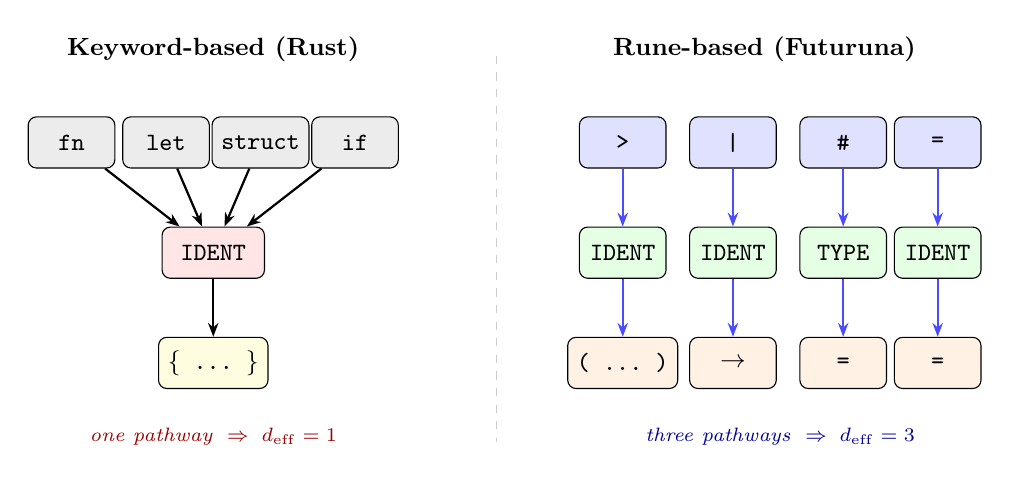
\begin{tikzpicture}[
    node distance=1.4cm and 1.8cm,
    every node/.style={font=\small},
    tok/.style={draw, rounded corners=3pt, minimum width=1.1cm, minimum height=0.65cm, font=\small\ttfamily},
    kw/.style={tok, fill=gray!15},
    sig/.style={tok, fill=blue!12},
    flow/.style={-{Stealth[length=5pt]}, thick},
    faint/.style={-{Stealth[length=4pt]}, gray!50, thin},
    label/.style={font=\small\bfseries, anchor=south},
]

% === LEFT PANEL: Keyword-based ===
\node[label] at (1.8, 3.1) {Keyword-based (Rust)};

\node[kw] (fn) at (0, 2.2) {fn};
\node[kw] (let) at (1.2, 2.2) {let};
\node[kw] (struct) at (2.4, 2.2) {struct};
\node[kw] (if) at (3.6, 2.2) {if};

% Bottleneck
\node[tok, fill=red!10, minimum width=1.3cm] (ident) at (1.8, 0.8) {IDENT};
\node[tok, fill=yellow!12] (brace) at (1.8, -0.6) {\{~\ldots~\}};

% All keywords funnel into IDENT
\draw[flow] (fn) -- (ident);
\draw[flow] (let) -- (ident);
\draw[flow] (struct) -- (ident);
\draw[flow] (if) -- (ident);
% IDENT funnels into braces
\draw[flow] (ident) -- (brace);

% Annotation
\node[font=\scriptsize\itshape, text=red!60!black, anchor=north] at (1.8, -1.3) {one pathway $\;\Rightarrow\; \deff = 1$};

% === RIGHT PANEL: Rune-based ===
\node[label] at (8.8, 3.1) {Rune-based (Futuruna)};

\node[sig] (gt) at (7.0, 2.2) {\texttt{>}};
\node[sig] (pipe) at (8.4, 2.2) {\texttt{|}};
\node[sig] (hash) at (9.8, 2.2) {\texttt{\#}};
\node[sig] (eq) at (11.0, 2.2) {\texttt{=}};

% Three distinct pathways
\node[tok, fill=green!10] (id1) at (7.0, 0.8) {IDENT};
\node[tok, fill=green!10] (id2) at (8.4, 0.8) {IDENT};
\node[tok, fill=green!10] (id3) at (9.8, 0.8) {TYPE};
\node[tok, fill=green!10] (id4) at (11.0, 0.8) {IDENT};

\node[tok, fill=orange!10] (paren) at (7.0, -0.6) {(~\ldots~)};
\node[tok, fill=orange!10] (arrow) at (8.4, -0.6) {$\rightarrow$};
\node[tok, fill=orange!10] (opeq) at (9.8, -0.6) {=};
\node[tok, fill=orange!10] (eqval) at (11.0, -0.6) {=};

% Diverging paths
\draw[flow, blue!70] (gt) -- (id1);
\draw[flow, blue!70] (id1) -- (paren);
\draw[flow, blue!70] (pipe) -- (id2);
\draw[flow, blue!70] (id2) -- (arrow);
\draw[flow, blue!70] (hash) -- (id3);
\draw[flow, blue!70] (id3) -- (opeq);
\draw[flow, blue!70] (eq) -- (id4);
\draw[flow, blue!70] (id4) -- (eqval);

% Annotation
\node[font=\scriptsize\itshape, text=blue!60!black, anchor=north] at (9.0, -1.3) {three pathways $\;\Rightarrow\; \deff = 3$};

% Divider
\draw[gray!40, dashed] (5.4, 3.3) -- (5.4, -1.6);

\end{tikzpicture}
\caption{\textbf{The bottleneck.} Keywords (left) funnel all statements through \texttt{IDENT} $\to$ \texttt{\{...\}}---one pathway, one dimension. Runes (right) create distinct chains (\texttt{>}~$\to$~\texttt{IDENT}~$\to$~\texttt{(...)}, \texttt{|}~$\to$~\texttt{IDENT}~$\to$~$\rightarrow$, \texttt{\#}~$\to$~\texttt{TYPE}~$\to$~\texttt{=}). Three independent pathways, three principal components, three cognitive dimensions.}
\label{fig:bottleneck}
\end{figure}

We ran NSGA-II \cite{Deb2002}, an evolutionary search that optimizes multiple goals at once, over the space of possible $22 \times 22$ transition matrices. The three goals: maximize optionality, clarity, and integration simultaneously. Population 500, 200 generations. The result was a Pareto frontier: the set of 122 designs where you cannot improve any one metric without worsening another. The best possible trade-offs.

85 of them achieve $\deff \geq 3$. All 85 share one structural feature: a strong \texttt{START} $\to$ \texttt{OP} transition. Statements begin with an operator, not a keyword.

\begin{claim}
Statement runes are necessary and sufficient for $\deff = 3$ in the measured token transition framework.
\end{claim}

No frontier member achieves $\deff = 3$ without them. Every member with them achieves $\deff \geq 3$.

Principal component analysis on the rune-based transition matrix finds three independent dimensions ($\lambda$: 2.28, 1.66, 0.96):

\begin{description}[nosep]
\item[Axis 1 --- Statement kind ($\lambda = 2.28$).] The rune at the start of each line. Your first cognitive act: \emph{what kind of statement is this?}

\item[Axis 2 --- Type flow ($\lambda = 1.66$).] Type signatures (\texttt{Int -> Bool -> String}) flow independently of statement kind. This axis exists in Haskell. In rune-based syntax, it decouples from Axis 1 because runes, not keywords, carry the statement's nature.

\item[Axis 3 --- Block composition ($\lambda = 0.96$).] How braces nest. In C-family languages this axis is entangled with Axis 1---keywords like \texttt{fn} and \texttt{class} initiate both statement kind \emph{and} block structure. Runes separate them.
\end{description}

Keywords overload two cognitive functions: they signal statement kind \emph{and} initiate blocks. The rune decouples these. The decoupling creates independence. The independence creates the third dimension.

%% ============================================================================
\section{Seven Runes}
%% ============================================================================

If runes unlock the third dimension, how many? The Pareto frontier constrains the answer: seven to nine produce the optimal balance of optionality, clarity, and integration. Seven is the sweet spot. They were not chosen by taste. They fell out of a question: \emph{what are the kinds of things a program can say?}

A program describes structures that can exist, processes that can happen, truths that must hold, facts that are observed, flows that evolve in time, boundaries where formal reasoning ends, and demands for verification.

Seven categories. Each gets a rune.

\begin{table}[H]
\centering
\caption{The seven runes of Futuruna. Each answers one epistemic question.}
\label{tab:runes}
\begin{tabular}{clll}
\toprule
Rune & Question & Verification target & Examples \\
\midrule
\texttt{\#} & What exists? & Z3 datatypes & Types, effects, traits \\
\texttt{>} & What happens? & Z3 functions & Functions, actors, modules \\
\texttt{|} & What must be true? & Z3 assertions & Rules, match arms, handlers \\
\texttt{=} & What is? & Z3 constants & Bindings, ground truth \\
\texttt{\textasciitilde} & What flows? & Temporal logic & Reactive streams, time \\
\texttt{@} & Where do proofs stop? & Proof boundary & IO, imports, meta \\
\texttt{?} & Prove it. & Solver invocation & Verification demands \\
\bottomrule
\end{tabular}
\end{table}

We conjecture this set is closed. Every proposed eighth rune we have tested reduces to one of these seven. Permissions are constraints on structures: \texttt{\#}. Concurrency is processes that happen in parallel: \texttt{>}. Error handling is case analysis: \texttt{|}. Macros are boundary operations: \texttt{@}. The seven-fold partition mirrors a natural decomposition of what programs express---ontology, dynamics, logic, observation, time, boundary, proof. We have not found a program statement that requires a genuinely new direction. Whether this partition is provably complete remains an open question; what we can show is that it covers every statement kind in the eight measured languages without overlap.

\subsection{\texttt{\#} --- What exists}

Types, algebraic effects, traits, implementations. In other languages, these are scattered across \texttt{class}, \texttt{struct}, \texttt{enum}, \texttt{interface}, \texttt{trait}, and \texttt{type}. In Futuruna, one rune:

\begin{lstlisting}
# List(T) = Nil | Cons(head: T, tail: List(T))
# Weather(temp: Float, condition: Condition, wind_kph: Float)

# effect Console {
    > say(msg: String) -> ()
    > ask(prompt: String) -> String
}

# trait Printable { > display(self) -> String }
\end{lstlisting}

\subsection{\texttt{>} --- What happens}

Functions, actors, modules. Everything that describes transformation:

\begin{lstlisting}
> add(a: Int, b: Int) -> Int { a + b }

> actor counter(state: Int) {
    | Increment -> state + 1
    | Decrement -> state - 1
}
\end{lstlisting}

\subsection{\texttt{=} --- What is}

Bindings. Ground truth. A point in time:

\begin{lstlisting}
= x = 42
= name = "hello"
= result <- parse_int("42")    -- monadic bind (unwrap or early-return)
\end{lstlisting}

\subsection{\texttt{\textasciitilde} --- What flows}

Where \texttt{=} binds a point in time, \texttt{\textasciitilde} binds a line through time:

\begin{lstlisting}
~ clicks = events("button", "click")
~ count = clicks |> scan(0, |n, _| n + 1)
~ label = count |> map(|n| "Count: " + show(n))
\end{lstlisting}

In every other language, reactive streams are a library---RxJS, Reactor, Akka Streams. In Futuruna, they are syntax. The compiler sees the stream topology at compile time.

\subsection{\texttt{@} --- Where proofs stop}

The boundary between the verified world and the effectful world. Every use of \texttt{@} says: \emph{here, formal reasoning cannot reach.}

\begin{lstlisting}
@ print("hello")                -- IO
@ use std::collections::HashMap -- external code
@ depend "serde" "1"            -- build system
@ comptime = table = gen(1000)  -- compile-time evaluation
@ rust { fn fast(x: &[f64]) { x.sort_unstable(); } }
\end{lstlisting}

\subsection{\texttt{?} --- Prove it}

At first glance, \texttt{?} seems simple: check a predicate, stop. The full picture is richer. Every other rune declares something. \texttt{?} interrogates it. The predicate comes from \texttt{>} and \texttt{|}. The subject comes from \texttt{\textasciitilde} and \texttt{=}. The reaction can use \texttt{@}. At each call site, the programmer decides: is violation fatal, recoverable, or informational?

Six forms, from simplest to most expressive. The key distinction: without an \texttt{else} block, failure halts the program. With an \texttt{else} block, failure is handled and execution continues.

\begin{lstlisting}
-- Bare check: halt on failure, continue on success
? balance_bounded

-- Pass block: run code on success, halt on failure
? balance_bounded -> { @ print("Balance OK") }

-- Capture + pass: bind the checked value, halt on failure
? balance_bounded: val -> { @ print("Value: " + show(val)) }

-- Else block: handle failure, no halt
? balance_bounded else { @ print("VIOLATION") }

-- Pass + else: handle both outcomes, no halt
? balance_bounded -> { @ print("OK") } else { @ print("FAIL") }

-- Full form: capture + pass + else, no halt
? balance_bounded: val -> {
    @ print("Verified: " + show(val))
} else {
    @ print("Violation detected")
}
\end{lstlisting}

You define what ``correct'' means declaratively, using \texttt{|} rules. Then at each call site you choose how to react. Without \texttt{else}, \texttt{?} is a hard assertion---failure stops the program. Add an \texttt{else} block and it becomes a recovery point---failure is handled, execution continues. The \texttt{: val} capture binds the subject value (the data being checked, not the boolean result), feeding verified data downstream. This is verification and error handling unified under one character.

The three assurance levels from the earlier section still apply to every form: \texttt{runa run} evaluates the predicate. \texttt{runa build} emits \texttt{debug\_assert!()}. \texttt{runa verify} invokes Z3 for a proof over all inputs. The shape of the reaction is independent of the depth of the proof.

%% ============================================================================
\section{A Complete Program}
%% ============================================================================

All seven runes in one file. Read the first character of each line as an epistemic declaration.

\begin{lstlisting}
# Phase = Idle | Active | Done

> add(a: Int, b: Int) -> Int { a + b }
> clamp(val: Int, lo: Int, hi: Int) -> Int {
    if val < lo { lo }
    else { if val > hi { hi } else { val } }
}

= x = 42
= y = 10
= balance = 1000
= max_supply = 1000000

| sum_positive: add(x, y) -> add(x, y) > 0
| balance_bounded: balance -> balance >= 0 && balance <= max_supply
| commutative: add(x, y) -> add(x, y) == add(y, x)

~ ticks = from_list([1, 2, 3, 4, 5])
~ evens = ticks |> filter(|n| n % 2 == 0)

@ print("--- Verifying ---")

? sum_positive
? balance_bounded: val -> { @ print("Balance: " + show(val)) }
? commutative else { @ print("Commutativity violated!") }
? all
\end{lstlisting}

\noindent Interpreter output:
\begin{verbatim}
--- Verifying ---
  [ok] |sum_positive| holds (value: 52)
  [ok] |balance_bounded| holds — Balance: 1000
  [ok] |commutative| holds (value: 52)
  [ok] all 3 invariant(s) hold
\end{verbatim}

Three different \texttt{?} forms in one program: a bare assertion, a value capture with a pass block, and an assertion with a recovery branch. With \texttt{runa verify}, all three invoke Z3 to prove each invariant for \emph{all} inputs. The reaction shape is orthogonal to the proof depth.

%% ============================================================================
\section{Measured Comparison}
%% ============================================================================

The number to watch is the last column.

\begin{table}[H]
\centering
\caption{Futuruna vs.\ existing languages. No existing language reaches $\deff = 3$.}
\label{tab:comparison}
\begin{tabular}{lccccc}
\toprule
Design & Optionality & Clarity & Integration & $\deff$ & Note \\
\midrule
Prolog & 2.891 & 0.688 & 0.937 & 2 & Most integrated among existing \\
Haskell & 3.012 & 0.671 & 0.883 & 2 & Best composite among existing \\
Scala & 3.115 & 0.589 & 0.412 & 1 & Most options among existing \\
Python & 2.743 & 0.749 & 0.621 & 1 & Clearest among existing \\
Rust & 2.987 & 0.634 & 0.000 & 1 & Zero integration \\
\midrule
\textbf{Futuruna} & \textbf{3.537} & \textbf{0.784} & \textbf{0.980} & \textbf{3} & Statement runes$^\dagger$ \\
\bottomrule
\end{tabular}

\smallskip
\noindent{\small $^\dagger$Futuruna metrics computed from the language's 30+ test programs. Production-scale codebases---where function bodies and bindings dominate---may produce different numbers. The structural claim ($\deff = 3$) rests on the rune mechanism, not the specific metric values.}
\end{table}

Futuruna dominates every measured language on all three axes simultaneously. More options than Scala. Clearer than Python. More integrated than Prolog. And the only design that reaches the third dimension.

What does this feel like? A Futuruna programmer scanning unfamiliar code has three questions answered before processing a single identifier. The rune says what \emph{kind} of statement. The type signatures say what \emph{types} flow through it. The block structure says where it \emph{sits}. Three facts, none redundant with the others, all arriving through separate visual cues that the brain processes in parallel.

Consider traffic signs. Imagine a city with no signs at all---just white text painted on the road surface. ``STOP.'' ``YIELD.'' ``SPEED LIMIT 50.'' Every instruction looks the same until you read the words. That is $\Phi = 0$: zero channels of pre-attentive information. You must decode every message. Now mount them on poles as round white signs with black text. You know something is a sign before you read it---that is $\deff = 1$: one channel (sign versus not-sign). Now add color: red means prohibition, blue means information, yellow means caution. You react to the color before you read the word. That is $\deff = 2$: two channels. Now add shape: octagons for stop, triangles for yield, rectangles for information. Shape, color, and text arrive on three parallel channels. You know what \emph{kind} of sign it is, what \emph{category} of instruction it carries, and what the \emph{specific} message says---all before conscious reading begins. That is $\deff = 3$.

Traffic signs work this way because the human visual system processes shape, color, and symbol on independent channels. Programming language syntax faces the same constraint: a programmer scanning unfamiliar code is a driver entering an unfamiliar intersection. Rust is the white text on asphalt---every line looks the same until you read the keyword. Futuruna is the shaped, colored sign: the rune tells you the kind, the type signature tells you the flow, and the block depth tells you the structure. Three questions, answered before conscious decoding begins.

%% ============================================================================
\section{The Formal Definitions}
%% ============================================================================

For completeness, the formal definitions behind the three named quantities.

\begin{definition}[Optionality $\Stau$]
For transition matrix $P$ with $(P)_{ij} = w(i,j) / \sum_k w(i,k)$:
\[
\Stau = \sum_i \pi_i \cdot H(P^\tau \cdot \delta_i), \quad \text{where} \quad H(\mathbf{p}) = -\sum_j p_j \log_2 p_j
\]
$\pi_i$ is the stationary weight of category $i$, $\delta_i$ is the unit vector at node $i$, $\tau = 3$.
\end{definition}

\begin{definition}[Clarity (JSD)]
\[
\mathrm{JSD} = \frac{1}{\binom{|V|}{2}} \sum_{i < j} \left[ \frac{1}{2} D_{\mathrm{KL}}(P_i \| M_{ij}) + \frac{1}{2} D_{\mathrm{KL}}(P_j \| M_{ij}) \right], \quad M_{ij} = \frac{P_i + P_j}{2}
\]
\end{definition}

\begin{definition}[Integration $\Phi$ and dimensionality $\deff$]
Let $C$ be the covariance matrix of the rows of $P$, with principal component variances $\lambda_1 \geq \lambda_2 \geq \dots$ Then:
\[
\deff = |\{ i : \lambda_i > \epsilon \}| \qquad \qquad \Phi = 1 - \frac{\lambda_1}{\sum_i \lambda_i}
\]
\end{definition}

%% ============================================================================
\section{Implementation}
%% ============================================================================

Futuruna is a 10{,}000+ line Rust compiler (\texttt{runa.rs}) with four modes:

\begin{description}[nosep]
\item[\texttt{runa run file.runa}] Interpret directly. \texttt{?} performs runtime checks.
\item[\texttt{runa emit file.runa}] Transpile to Rust, display generated code.
\item[\texttt{runa build file.runa}] Transpile to Rust, compile to native binary.
\item[\texttt{runa verify file.runa}] Invoke Z3 for formal proofs of all invariants.
\end{description}

\subsection{Ownership without annotation}

Futuruna is to Rust as Kotlin is to Java. The programmer writes value semantics; the compiler handles ownership. Whole-program escape analysis decides: single-use variables move, multi-use variables clone, read-only parameters auto-borrow. The programmer never writes \texttt{\&T}, never annotates a lifetime, never calls \texttt{.clone()}. An escape hatch (\texttt{@ rust \{\}}) covers the remaining 5\%.

\subsection{The verification pipeline}

The runes are not decoration. They are the interface to the verifier. Each maps directly to a category in the standard theorem-prover input format (SMT-LIB2):

\begin{itemize}[nosep]
\item \texttt{\#} algebraic types $\to$ \texttt{declare-datatypes}
\item \texttt{>} functions $\to$ \texttt{define-fun}
\item \texttt{=} bindings $\to$ \texttt{define-const}
\item \texttt{|} invariants $\to$ assert $\neg$predicate (refutation)
\end{itemize}

The seven runes partition a program into exactly the categories a formal methods tool needs. The syntax \emph{is} the verification interface.

%% ============================================================================
\section{Honest Limitations}
%% ============================================================================

\begin{itemize}[nosep]
\item \textbf{The metrics are proxies.} Optionality, clarity, and integration measure syntactic texture, not programmer productivity. Three cognitive axes \emph{should} improve the experience of reading code, but this has not been tested in user studies. The metrics are a map, not the territory.

\item \textbf{Corpus dependence.} Transition matrices depend on which code samples represent each language. Systems code and web code produce different numbers. Representativeness is inherently debatable.

\item \textbf{Verification scope.} The \texttt{--verify} pipeline handles integer arithmetic, algebraic data types, and first-order functions. Higher-order functions and floating-point require extensions not yet shipped.

\item \textbf{Reactive streams.} The \texttt{\textasciitilde} rune supports both synchronous \texttt{Vec}-based and asynchronous multi-threaded semantics. Timing operators (debounce, throttle) are not yet implemented.

\item \textbf{Maturity.} Futuruna is a working compiler with 30+ test programs, not a production language. The escape hatch covers the gaps.
\end{itemize}

The deepest limitation is the first. We measured the information-theoretic structure of token transition graphs and found something real. Whether the third cognitive dimension translates to the lived experience of writing code is an empirical question this paper opens but does not close.

The strongest version of this work's contribution is not ``Futuruna is better'' but ``measurement reveals structure that intuition missed.'' If someone builds a better language using different measurements, the methodology wins.

%% ============================================================================
\section{Related Work}
%% ============================================================================

\textbf{Integrated Information Theory} \cite{Tononi2004} provides the framework for integration ($\Phi$). Tononi developed IIT to formalize consciousness in neural systems; we apply it to the covariance structure of token transitions. \textbf{Causal entropic forces} \cite{WissnerGross2013} provide optionality ($\Stau$); Wissner-Gross and Freer showed that maximizing path entropy produces intelligent behavior in physical systems; we show it characterizes syntactic freedom.

\textbf{Catala} \cite{Merigoux2021} pioneered legal default logic; Futuruna absorbs this into \texttt{|}. \textbf{Koka} \cite{Leijen2017} proved algebraic effects are tractable; Futuruna adopts them via \texttt{\# effect} and \texttt{| handle}. \textbf{Unison} \cite{Chiusano2019} showed content-addressed code eliminates dependency hell; Futuruna implements it via AST hashing. \textbf{Zig} demonstrated compile-time evaluation eliminates macros; Futuruna adopts \texttt{@ comptime}. \textbf{Hylo} explored mutable value semantics; Futuruna adopts \texttt{inout}.

No prior language has combined these features, and none has derived its syntax from quantitative measurement.

%% ============================================================================
\section{Conclusion}
%% ============================================================================

We measured the cognitive structure of programming language syntax and found that every existing language occupies at most two dimensions. A third dimension is available. It requires a constraint that is not the one intuition suggests.

Not richness. Not flexibility. Not multi-paradigm abundance.

Differentiation.

One character at the start of each line that says: \emph{this is what kind of thing I am about to tell you.} Seven characters, covering every category of program statement we have found. Each one maps to a verification target. Each one creates a distinct cognitive pathway.

The language that results unifies things that have never coexisted: logic programming and algebraic effects and legal default logic and reactive streams, all under a syntax that sits on the Pareto frontier for the information-theoretic proxies we have. You cannot improve one metric without worsening another. It compiles to native Rust with inferred ownership. It provides formal verification through the same runes that structure the code. And it occupies a region of the design space that no existing language has reached.

Remember the feeling from the first paragraph. You open a file and within seconds you know whether you are in friendly territory. That feeling has a name now. It is $\deff$---the number of questions the syntax answers before you read a single word.

Every existing language leaves at least one of those questions unanswered.

\begin{thebibliography}{99}

\bibitem{Shannon1948}
C.~E. Shannon.
\newblock A mathematical theory of communication.
\newblock {\em Bell System Technical Journal}, 27(3):379--423, 1948.

\bibitem{WissnerGross2013}
A.~D. Wissner-Gross and C.~E. Freer.
\newblock Causal entropic forces.
\newblock {\em Physical Review Letters}, 110:168702, 2013.

\bibitem{Tononi2004}
G.~Tononi.
\newblock An information integration theory of consciousness.
\newblock {\em BMC Neuroscience}, 5:42, 2004.

\bibitem{Merigoux2021}
D.~M\'erigoux, N.~Chataing, and J.~Protzenko.
\newblock Catala: A programming language for the law.
\newblock {\em Proc.\ ACM on Programming Languages}, 5(ICFP):1--29, 2021.

\bibitem{Leijen2017}
D.~Leijen.
\newblock Type directed compilation of row-typed algebraic effects.
\newblock In {\em Proc.\ POPL}, pages 486--499, 2017.

\bibitem{Chiusano2019}
P.~Chiusano and R.~Bjarnason.
\newblock Unison: a new approach to distributed programming.
\newblock \url{https://www.unison-lang.org/}, 2019.

\bibitem{Deb2002}
K.~Deb, A.~Pratap, S.~Agarwal, and T.~Meyarivan.
\newblock A fast and elitist multiobjective genetic algorithm: {NSGA-II}.
\newblock {\em IEEE Trans.\ Evolutionary Computation}, 6(2):182--197, 2002.

\bibitem{DeMoura2008}
L.~de~Moura and N.~Bj{\o}rner.
\newblock {Z3}: An efficient {SMT} solver.
\newblock In {\em Proc.\ TACAS}, pages 337--340, 2008.

\end{thebibliography}

\end{document}
